\subsection{Atomic structure of Alkali atoms}
In these experiments, we will study the absorption of light by rubidium atoms. In the
quantum mechanical model we consider, atoms are described in terms of the
\textbf{central field approximation}, in which the nucleus is taken to be a point particle
characterized by its charge, spin angular momentum, and electric and magnetic moments.
The energy levels can be described by angular momentum wave functions calculated from
the angular parts of the separated Schr\"{o}dinger equation, and a perturbation theory
approach is used to obtain the eigenstates of the atom. For alkali atoms, the angular
momenta are coupled in the \textbf{Russell-Saunders coupling scheme}.
 
All alkali atoms are similar in structure to the hydrogen atom : many of their properties are
determined by a single valence electron. Rubidium, with atomic number 37, has the
electronic configuration :
\begin{equation}
    1s^2\,2s^2\,2p^6\,3s^2\,3p^6\,3d^{10}\,4s^2\,4p^6\,5s
\end{equation}
Since the electrons in the inner shells are paired, we can neglect their presence entirely and
focus on the single outer electron. The entire discussion of the optical pumping experiments
is therefore based on a model that treats a free rubidium atom as a simple hydrogenic
single-electron atom.
 
\subsubsection*{Fine Structure}
 
The outer electron is described by an orbital angular momentum $L$, a spin angular
momentum $S$, and a total non-nuclear angular momentum $J$, all in units of $\hbar$ :
\begin{equation}
    \mathbf{J} = \mathbf{L} + \mathbf{S}
\end{equation}
Each of these angular momenta has a magnetic dipole moment associated with it, and they
are coupled by a magnetic interaction of the form $\boldsymbol{\mu}_L \cdot \boldsymbol{\mu}_S$.
In the absence of further interactions, $\mathbf{J}$ is a constant of the motion.
 
In the electronic ground state of an alkali atom, $L = 0$ (as in hydrogen). Since a single
electron has intrinsic spin $S = \tfrac{1}{2}$, the total angular momentum is $J = \tfrac{1}{2}$.
In spectroscopic notation $^{2S+1}L_J$, this ground state is designated $^2S_{1/2}$.
 
The first excited state has $L = 1$ (a P state). Since $J$ can only take the values
$L + S$ and $L - S$, there are two excited states : $^2P_{1/2}$ and $^2P_{3/2}$. These
states have different energies — the energy splitting between them is called the
\textbf{Fine Structure}. Note that the fine structure splitting is much smaller than the
energy difference between the ground state and the first excited state.
 
\subsubsection*{Hyperfine Structure}
 
We must also take into account the nuclear spin $I$ and the nuclear magnetic dipole moment.
The nuclear moment couples with the electronic magnetic dipole moment associated with
$\mathbf{J}$ to form the total angular momentum of the atom $\mathbf{F}$ :
\begin{equation}
    \mathbf{F} = \mathbf{I} + \mathbf{J}
\end{equation}
This interaction, of the form $\boldsymbol{\mu}_I \cdot \boldsymbol{\mu}_J$, produces a
further splitting of the energy levels called the \textbf{Hyperfine Structure}. It is
characterized by the Hamiltonian :
\begin{equation}
    H = ha\,\mathbf{I} \cdot \mathbf{J}
\end{equation}
where $h$ is Planck's constant and $a$ is a constant that is different for each electronic
state and is determined experimentally. For a nuclear spin $I = \tfrac{3}{2}$, the
hyperfine interaction splits each fine-structure level into two levels with
$F = I + J$ and $F = |I - J|$, as shown schematically in figure below.

\begin{figure}[H]
    \centering
    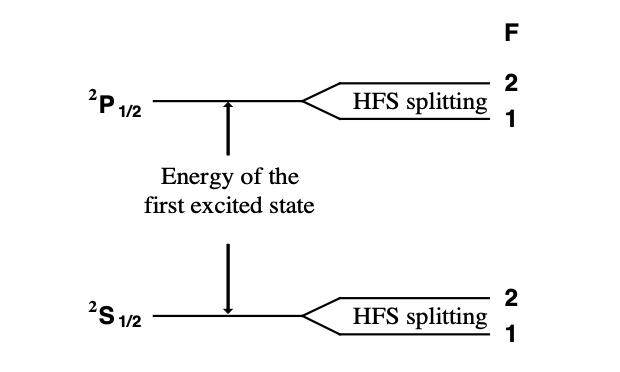
\includegraphics[width=0.5\linewidth]{theory pics/theory 1 pic.png}
    \caption{Hyperfine structure of I = 3/2}
\end{figure}
